\documentclass{standalone}
\usepackage{tikz}
\usetikzlibrary{patterns, positioning}
\usepackage[sfdefault]{ClearSans} %% option 'sfdefault' activates Clear Sans as the default text font
\usepackage[T1]{fontenc}

\begin{document}
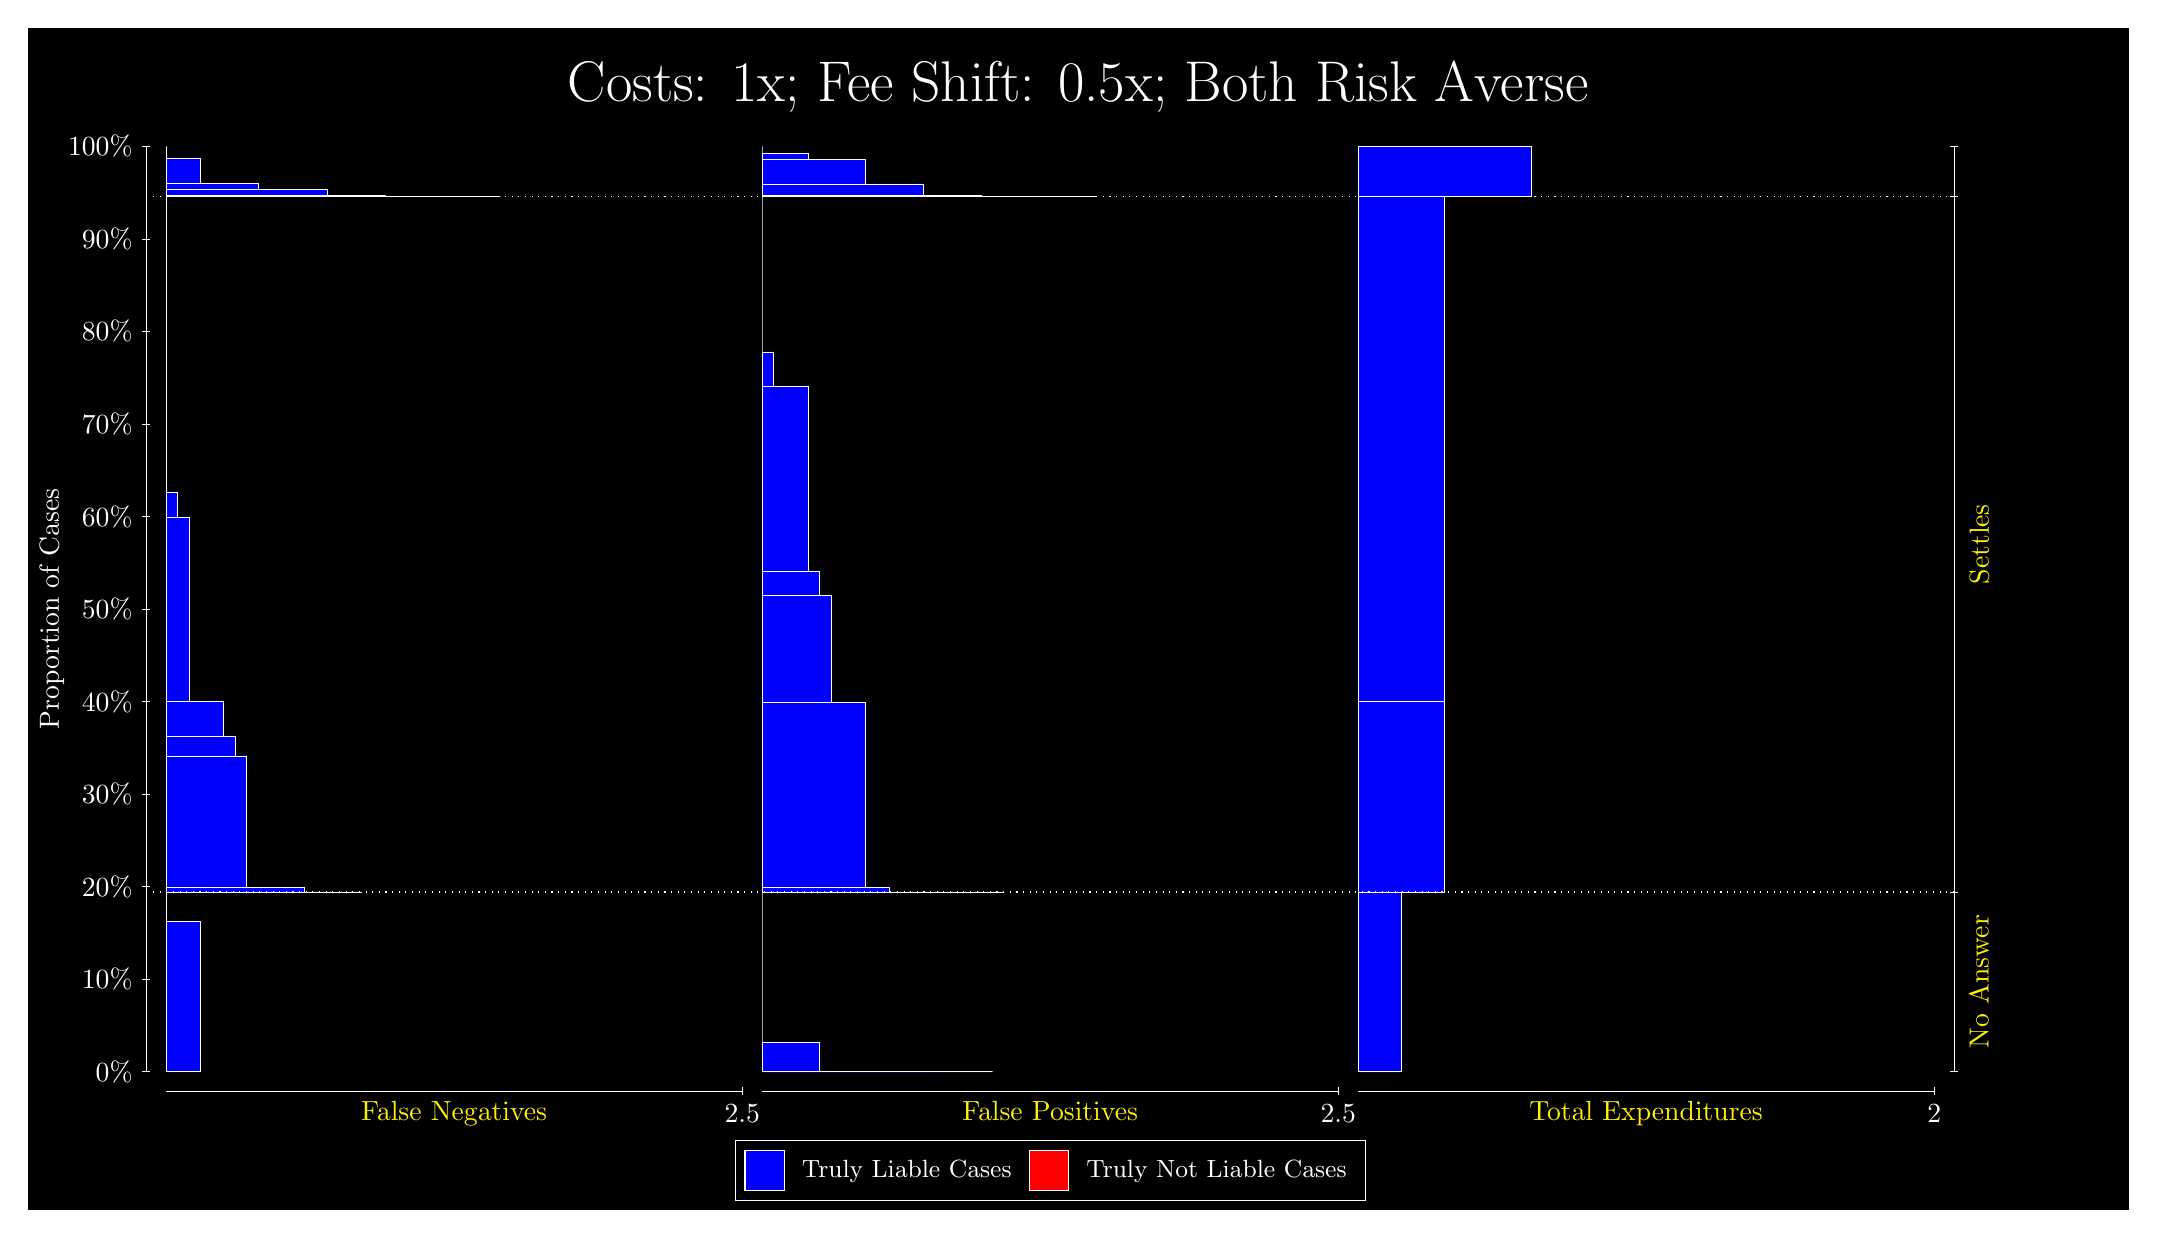
\begin{tikzpicture}
\draw[fill=black] (0,0) rectangle (26.667,15);
\draw[text=white] (0,13.5) rectangle (26.667,15) node[midway] {\huge Costs: 1x; Fee Shift: 0.5x; Both Risk Averse};
\draw[white, very thin] (1.5,1.75) -- (1.5,13.5);
\node[rotate=90, text=white, anchor=center] at (0.3, 7.625) {Proportion of Cases};
\draw[white, very thin] (1.45,1.75) -- (1.55,1.75);
\node[text=white, anchor=east] at (1.45, 1.75) {0\%};
\draw[white, very thin] (1.45,2.925) -- (1.55,2.925);
\node[text=white, anchor=east] at (1.45, 2.925) {10\%};
\draw[white, very thin] (1.45,4.1) -- (1.55,4.1);
\node[text=white, anchor=east] at (1.45, 4.1) {20\%};
\draw[white, very thin] (1.45,5.275) -- (1.55,5.275);
\node[text=white, anchor=east] at (1.45, 5.275) {30\%};
\draw[white, very thin] (1.45,6.45) -- (1.55,6.45);
\node[text=white, anchor=east] at (1.45, 6.45) {40\%};
\draw[white, very thin] (1.45,7.625) -- (1.55,7.625);
\node[text=white, anchor=east] at (1.45, 7.625) {50\%};
\draw[white, very thin] (1.45,8.8) -- (1.55,8.8);
\node[text=white, anchor=east] at (1.45, 8.8) {60\%};
\draw[white, very thin] (1.45,9.975) -- (1.55,9.975);
\node[text=white, anchor=east] at (1.45, 9.975) {70\%};
\draw[white, very thin] (1.45,11.15) -- (1.55,11.15);
\node[text=white, anchor=east] at (1.45, 11.15) {80\%};
\draw[white, very thin] (1.45,12.325) -- (1.55,12.325);
\node[text=white, anchor=east] at (1.45, 12.325) {90\%};
\draw[white, very thin] (1.45,13.5) -- (1.55,13.5);
\node[text=white, anchor=east] at (1.45, 13.5) {100\%};

\draw[white, very thin] (24.457,1.75) -- (24.457,13.5);
\draw[white, very thin] (24.407,1.75) -- (24.507,1.75);
\node[anchor=west] at (24.407, 1.75) {};
\draw[white, very thin] (24.407,4.0302) -- (24.507,4.0302);
\node[anchor=west] at (24.407, 4.0302) {};
\draw[white, very thin] (24.407,12.865) -- (24.507,12.865);
\node[anchor=west] at (24.407, 12.865) {};
\draw[white, very thin] (24.407,13.5) -- (24.507,13.5);
\node[anchor=west] at (24.407, 13.5) {};

\draw[white, very thin, fill=blue] (1.75,1.75) rectangle (2.1891,3.6568);
\draw[white, very thin, fill=red] (1.75,3.6568) rectangle (1.75,3.6568);
\draw[white, very thin, fill=blue] (1.75,3.6568) rectangle (1.75,4.0302);
\draw[white, very thin, fill=blue] (1.75,4.0302) rectangle (4.2384,4.0302);
\draw[white, very thin, fill=blue] (1.75,4.0302) rectangle (3.5065,4.0895);
\draw[white, very thin, fill=blue] (1.75,4.0895) rectangle (3.3602,4.0902);
\draw[white, very thin, fill=blue] (1.75,4.0902) rectangle (2.7746,5.7537);
\draw[white, very thin, fill=blue] (1.75,5.7537) rectangle (2.6283,6.0089);
\draw[white, very thin, fill=blue] (1.75,6.0089) rectangle (2.4819,6.4476);
\draw[white, very thin, fill=blue] (1.75,6.4476) rectangle (2.0428,8.7912);
\draw[white, very thin, fill=blue] (1.75,8.7912) rectangle (1.8964,9.1023);
\draw[white, very thin, fill=red] (1.75,9.1023) rectangle (1.75,9.1023);
\draw[white, very thin, fill=blue] (1.75,9.1023) rectangle (1.75,12.865);
\draw[white, very thin, fill=blue] (1.75,12.865) rectangle (5.9949,12.865);
\draw[white, very thin, fill=blue] (1.75,12.865) rectangle (5.2631,12.865);
\draw[white, very thin, fill=blue] (1.75,12.865) rectangle (4.5312,12.88);
\draw[white, very thin, fill=blue] (1.75,12.88) rectangle (3.7993,12.953);
\draw[white, very thin, fill=blue] (1.75,12.953) rectangle (3.6529,12.953);
\draw[white, very thin, fill=blue] (1.75,12.953) rectangle (3.0674,12.954);
\draw[white, very thin, fill=blue] (1.75,12.954) rectangle (2.921,13.029);
\draw[white, very thin, fill=blue] (1.75,13.029) rectangle (2.3355,13.029);
\draw[white, very thin, fill=blue] (1.75,13.029) rectangle (2.1891,13.346);
\draw[white, very thin, fill=red] (1.75,13.346) rectangle (1.75,13.346);
\draw[white, very thin, fill=blue] (1.75,13.346) rectangle (1.75,13.5);
\draw[white, very thin, fill=red] (9.3189,1.75) rectangle (12.246,1.75);
\draw[white, very thin, fill=blue] (9.3189,1.75) rectangle (12.246,1.75);
\draw[white, very thin, fill=blue] (9.3189,1.75) rectangle (11.515,1.75);
\draw[white, very thin, fill=blue] (9.3189,1.75) rectangle (10.783,1.7532);
\draw[white, very thin, fill=blue] (9.3189,1.7532) rectangle (10.051,2.1234);
\draw[white, very thin, fill=blue] (9.3189,2.1234) rectangle (9.3189,4.0302);
\draw[white, very thin, fill=red] (9.3189,4.0302) rectangle (12.393,4.0302);
\draw[white, very thin, fill=blue] (9.3189,4.0302) rectangle (12.393,4.0302);
\draw[white, very thin, fill=blue] (9.3189,4.0302) rectangle (11.661,4.0302);
\draw[white, very thin, fill=red] (9.3189,4.0302) rectangle (11.515,4.0302);
\draw[white, very thin, fill=blue] (9.3189,4.0302) rectangle (11.515,4.0302);
\draw[white, very thin, fill=blue] (9.3189,4.0302) rectangle (10.929,4.0888);
\draw[white, very thin, fill=blue] (9.3189,4.0888) rectangle (10.783,4.092);
\draw[white, very thin, fill=red] (9.3189,4.092) rectangle (10.636,4.092);
\draw[white, very thin, fill=blue] (9.3189,4.092) rectangle (10.636,6.442);
\draw[white, very thin, fill=blue] (9.3189,6.442) rectangle (10.197,7.7933);
\draw[white, very thin, fill=blue] (9.3189,7.7933) rectangle (10.051,8.1043);
\draw[white, very thin, fill=blue] (9.3189,8.1043) rectangle (9.9044,10.448);
\draw[white, very thin, fill=blue] (9.3189,10.448) rectangle (9.4652,10.887);
\draw[white, very thin, fill=blue] (9.3189,10.887) rectangle (9.3189,12.865);
\draw[white, very thin, fill=red] (9.3189,12.865) rectangle (13.564,12.865);
\draw[white, very thin, fill=blue] (9.3189,12.865) rectangle (13.564,12.865);
\draw[white, very thin, fill=red] (9.3189,12.865) rectangle (12.832,12.865);
\draw[white, very thin, fill=blue] (9.3189,12.865) rectangle (12.832,12.865);
\draw[white, very thin, fill=red] (9.3189,12.865) rectangle (12.1,12.865);
\draw[white, very thin, fill=blue] (9.3189,12.865) rectangle (12.1,12.872);
\draw[white, very thin, fill=blue] (9.3189,12.872) rectangle (11.368,13.019);
\draw[white, very thin, fill=blue] (9.3189,13.019) rectangle (10.636,13.336);
\draw[white, very thin, fill=red] (9.3189,13.336) rectangle (10.49,13.336);
\draw[white, very thin, fill=blue] (9.3189,13.336) rectangle (10.49,13.336);
\draw[white, very thin, fill=blue] (9.3189,13.336) rectangle (9.9044,13.411);
\draw[white, very thin, fill=blue] (9.3189,13.411) rectangle (9.758,13.413);
\draw[white, very thin, fill=red] (9.3189,13.413) rectangle (9.758,13.413);
\draw[white, very thin, fill=blue] (9.3189,13.413) rectangle (9.758,13.413);
\draw[white, very thin, fill=blue] (9.3189,13.413) rectangle (9.3189,13.5);
\draw[white, very thin, fill=red] (16.888,1.75) rectangle (17.437,1.75);
\draw[white, very thin, fill=blue] (16.888,1.75) rectangle (17.437,4.0302);
\draw[white, very thin, fill=red] (16.888,4.0302) rectangle (17.986,4.0302);
\draw[white, very thin, fill=blue] (16.888,4.0302) rectangle (17.986,6.4489);
\draw[white, very thin, fill=red] (16.888,6.4489) rectangle (17.986,6.4489);
\draw[white, very thin, fill=blue] (16.888,6.4489) rectangle (17.986,12.865);
\draw[white, very thin, fill=red] (16.888,12.865) rectangle (19.083,12.865);
\draw[white, very thin, fill=blue] (16.888,12.865) rectangle (19.083,13.5);
\draw[white, dotted] (1.5,4.0302) -- (24.457,4.0302);
\draw[white, dotted] (1.5,12.865) -- (24.457,12.865);
\draw[white, very thin] (1.75,1.5) -- (9.0689,1.5);
\node[text=yellow, anchor=north] at (5.4094, 1.5) {False Negatives};
\draw[white, very thin] (9.0689,1.45) -- (9.0689,1.55);
\node[text=white, anchor=north] at (9.0689, 1.45) {2.5};

\draw[white, very thin] (9.3189,1.5) -- (16.638,1.5);
\node[text=yellow, anchor=north] at (12.978, 1.5) {False Positives};
\draw[white, very thin] (16.638,1.45) -- (16.638,1.55);
\node[text=white, anchor=north] at (16.638, 1.45) {2.5};

\draw[white, very thin] (16.888,1.5) -- (24.207,1.5);
\node[text=yellow, anchor=north] at (20.547, 1.5) {Total Expenditures};
\draw[white, very thin] (24.207,1.45) -- (24.207,1.55);
\node[text=white, anchor=north] at (24.207, 1.45) {2};

\node[text=yellow, centered, rotate=90] at (24.777, 2.8901) {No Answer};
\node[text=yellow, centered, rotate=90] at (24.777, 8.4478) {Settles};


\draw (12.978300999999998,1.5) node[draw=none] (baseCoordinate) {};
\begin{scope}[align=center]
        \matrix[scale=0.5, draw=white, below=0.5cm of baseCoordinate, nodes={draw}, column sep=0.1cm]{
            \node[rectangle, draw, minimum width=0.5cm, minimum height=0.5cm, fill=blue] {}; &
            \node[draw=none, font=\small, text=white] (B) {Truly Liable Cases}; &
            \node[rectangle, draw, minimum width=0.5cm, minimum height=0.5cm, fill=red] {}; &
            \node[draw=none, font=\small, text=white] (B) {Truly Not Liable Cases}; \\
            };
\end{scope}

\end{tikzpicture}
\end{document}